% Created by tikzDevice version 0.7.0 on 2014-07-24 03:37:39
% !TEX encoding = UTF-8 Unicode
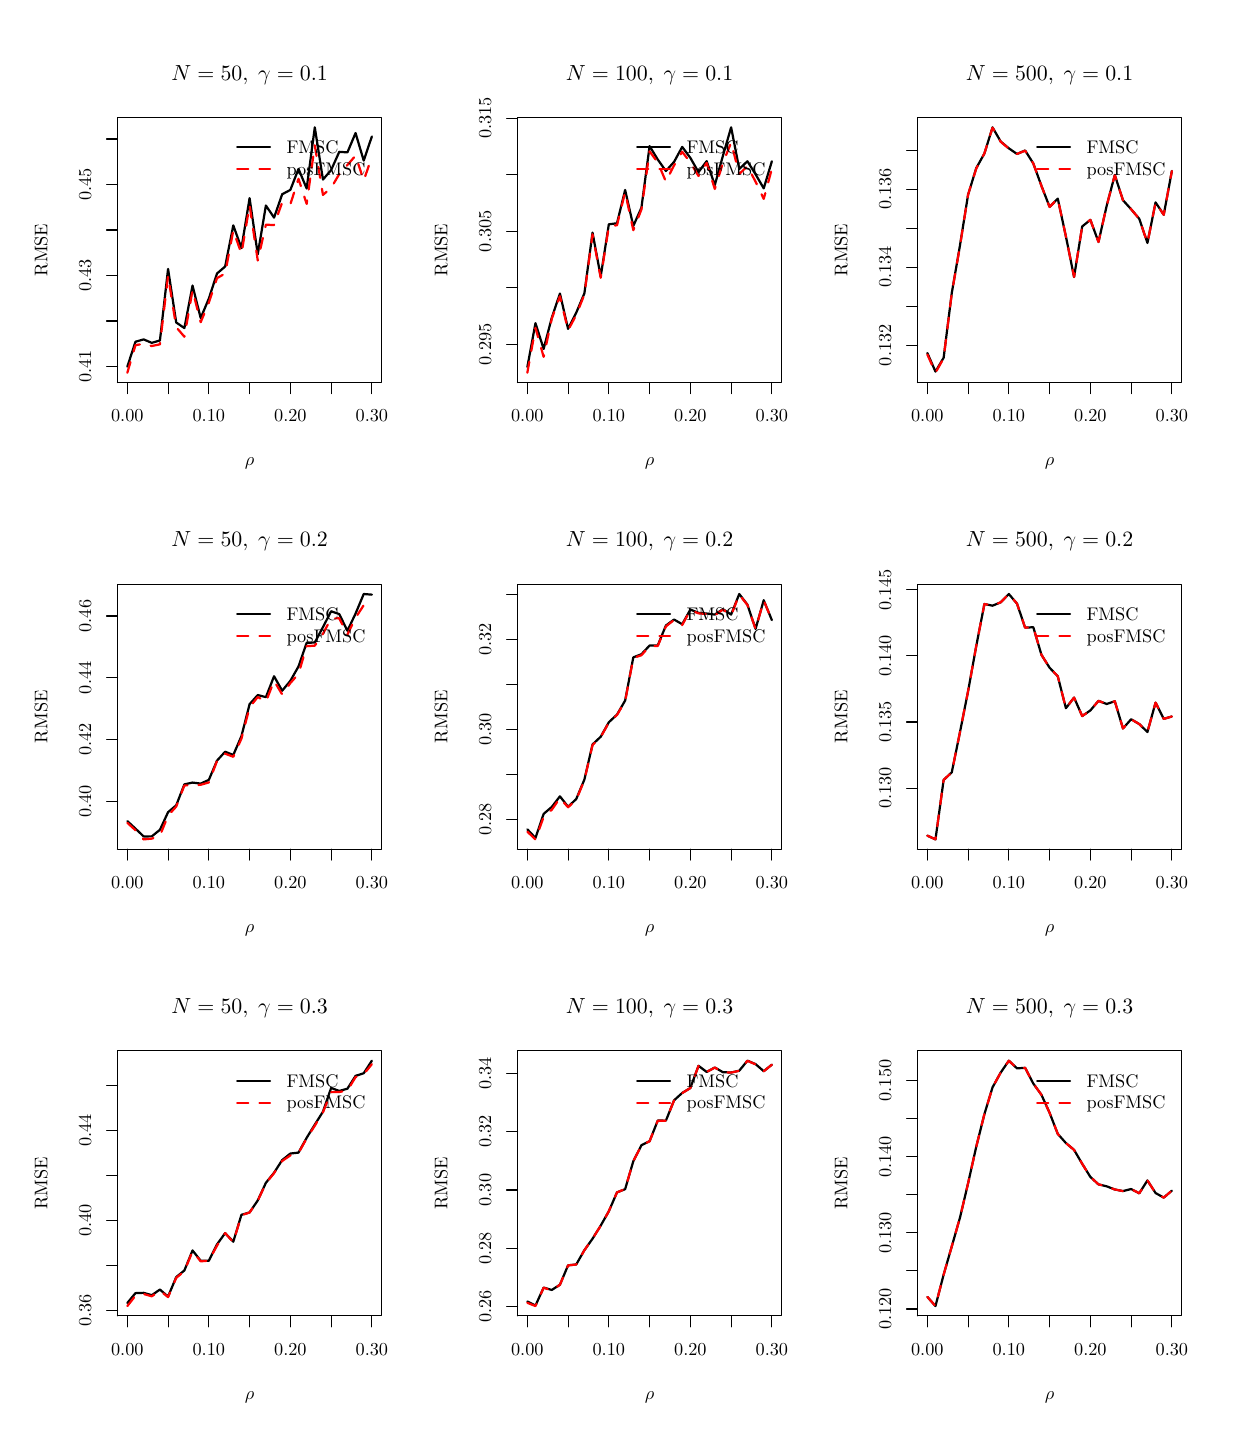
\begin{tikzpicture}[x=1pt,y=1pt]
\definecolor[named]{fillColor}{rgb}{1.00,1.00,1.00}
\path[use as bounding box,fill=fillColor,fill opacity=0.00] (0,0) rectangle (433.62,505.89);
\begin{scope}
\path[clip] ( 32.47,377.65) rectangle (127.91,473.42);
\definecolor[named]{drawColor}{rgb}{0.00,0.00,0.00}

\path[draw=drawColor,line width= 0.8pt,line join=round,line cap=round] ( 36.01,383.38) --
	( 38.95,392.40) --
	( 41.90,393.24) --
	( 44.84,392.00) --
	( 47.79,392.85) --
	( 50.73,418.71) --
	( 53.68,399.33) --
	( 56.63,397.35) --
	( 59.57,412.69) --
	( 62.52,400.97) --
	( 65.46,407.99) --
	( 68.41,417.05) --
	( 71.35,419.57) --
	( 74.30,434.44) --
	( 77.24,426.24) --
	( 80.19,444.29) --
	( 83.14,423.98) --
	( 86.08,441.61) --
	( 89.03,437.25) --
	( 91.97,445.70) --
	( 94.92,447.26) --
	( 97.86,454.85) --
	(100.81,447.77) --
	(103.75,469.87) --
	(106.70,451.00) --
	(109.65,454.42) --
	(112.59,461.02) --
	(115.54,460.82) --
	(118.48,467.81) --
	(121.43,457.85) --
	(124.37,466.57);
\end{scope}
\begin{scope}
\path[clip] (  0.00,  0.00) rectangle (433.62,505.89);
\definecolor[named]{drawColor}{rgb}{0.00,0.00,0.00}

\path[draw=drawColor,line width= 0.4pt,line join=round,line cap=round] ( 36.01,377.65) -- (124.37,377.65);

\path[draw=drawColor,line width= 0.4pt,line join=round,line cap=round] ( 36.01,377.65) -- ( 36.01,373.69);

\path[draw=drawColor,line width= 0.4pt,line join=round,line cap=round] ( 50.73,377.65) -- ( 50.73,373.69);

\path[draw=drawColor,line width= 0.4pt,line join=round,line cap=round] ( 65.46,377.65) -- ( 65.46,373.69);

\path[draw=drawColor,line width= 0.4pt,line join=round,line cap=round] ( 80.19,377.65) -- ( 80.19,373.69);

\path[draw=drawColor,line width= 0.4pt,line join=round,line cap=round] ( 94.92,377.65) -- ( 94.92,373.69);

\path[draw=drawColor,line width= 0.4pt,line join=round,line cap=round] (109.65,377.65) -- (109.65,373.69);

\path[draw=drawColor,line width= 0.4pt,line join=round,line cap=round] (124.37,377.65) -- (124.37,373.69);

\node[text=drawColor,anchor=base,inner sep=0pt, outer sep=0pt, scale=  0.66] at ( 36.01,363.40) {0.00};

\node[text=drawColor,anchor=base,inner sep=0pt, outer sep=0pt, scale=  0.66] at ( 65.46,363.40) {0.10};

\node[text=drawColor,anchor=base,inner sep=0pt, outer sep=0pt, scale=  0.66] at ( 94.92,363.40) {0.20};

\node[text=drawColor,anchor=base,inner sep=0pt, outer sep=0pt, scale=  0.66] at (124.37,363.40) {0.30};

\path[draw=drawColor,line width= 0.4pt,line join=round,line cap=round] ( 32.47,383.43) -- ( 32.47,465.65);

\path[draw=drawColor,line width= 0.4pt,line join=round,line cap=round] ( 32.47,383.43) -- ( 28.51,383.43);

\path[draw=drawColor,line width= 0.4pt,line join=round,line cap=round] ( 32.47,399.88) -- ( 28.51,399.88);

\path[draw=drawColor,line width= 0.4pt,line join=round,line cap=round] ( 32.47,416.32) -- ( 28.51,416.32);

\path[draw=drawColor,line width= 0.4pt,line join=round,line cap=round] ( 32.47,432.76) -- ( 28.51,432.76);

\path[draw=drawColor,line width= 0.4pt,line join=round,line cap=round] ( 32.47,449.20) -- ( 28.51,449.20);

\path[draw=drawColor,line width= 0.4pt,line join=round,line cap=round] ( 32.47,465.65) -- ( 28.51,465.65);

\node[text=drawColor,rotate= 90.00,anchor=base,inner sep=0pt, outer sep=0pt, scale=  0.66] at ( 22.97,383.43) {0.41};

\node[text=drawColor,rotate= 90.00,anchor=base,inner sep=0pt, outer sep=0pt, scale=  0.66] at ( 22.97,416.32) {0.43};

\node[text=drawColor,rotate= 90.00,anchor=base,inner sep=0pt, outer sep=0pt, scale=  0.66] at ( 22.97,449.20) {0.45};

\path[draw=drawColor,line width= 0.4pt,line join=round,line cap=round] ( 32.47,377.65) --
	(127.91,377.65) --
	(127.91,473.42) --
	( 32.47,473.42) --
	( 32.47,377.65);
\end{scope}
\begin{scope}
\path[clip] (  0.00,337.26) rectangle (144.54,505.89);
\definecolor[named]{drawColor}{rgb}{0.00,0.00,0.00}

\node[text=drawColor,anchor=base,inner sep=0pt, outer sep=0pt, scale=  0.79] at ( 80.19,486.92) {\bfseries $N=50, \;\gamma=0.1$};

\node[text=drawColor,anchor=base,inner sep=0pt, outer sep=0pt, scale=  0.66] at ( 80.19,347.56) {$\rho$};

\node[text=drawColor,rotate= 90.00,anchor=base,inner sep=0pt, outer sep=0pt, scale=  0.66] at (  7.13,425.54) {RMSE};
\end{scope}
\begin{scope}
\path[clip] ( 32.47,377.65) rectangle (127.91,473.42);
\definecolor[named]{drawColor}{rgb}{1.00,0.00,0.00}

\path[draw=drawColor,line width= 0.8pt,dash pattern=on 4pt off 4pt ,line join=round,line cap=round] ( 36.01,381.20) --
	( 38.95,391.17) --
	( 41.90,391.65) --
	( 44.84,390.85) --
	( 47.79,391.46) --
	( 50.73,416.20) --
	( 53.68,397.66) --
	( 56.63,394.20) --
	( 59.57,411.00) --
	( 62.52,399.46) --
	( 65.46,406.54) --
	( 68.41,415.37) --
	( 71.35,417.05) --
	( 74.30,432.61) --
	( 77.24,424.21) --
	( 80.19,441.69) --
	( 83.14,421.74) --
	( 86.08,434.69) --
	( 89.03,434.56) --
	( 91.97,442.75) --
	( 94.92,442.08) --
	( 97.86,451.26) --
	(100.81,442.21) --
	(103.75,463.36) --
	(106.70,445.46) --
	(109.65,447.98) --
	(112.59,452.99) --
	(115.54,456.26) --
	(118.48,459.65) --
	(121.43,450.63) --
	(124.37,459.19);
\definecolor[named]{drawColor}{rgb}{0.00,0.00,0.00}

\path[draw=drawColor,line width= 0.8pt,line join=round,line cap=round] ( 75.72,462.63) -- ( 87.60,462.63);
\definecolor[named]{drawColor}{rgb}{1.00,0.00,0.00}

\path[draw=drawColor,line width= 0.8pt,dash pattern=on 4pt off 4pt ,line join=round,line cap=round] ( 75.72,454.71) -- ( 87.60,454.71);
\definecolor[named]{drawColor}{rgb}{0.00,0.00,0.00}

\node[text=drawColor,anchor=base west,inner sep=0pt, outer sep=0pt, scale=  0.66] at ( 93.54,460.35) {FMSC};

\node[text=drawColor,anchor=base west,inner sep=0pt, outer sep=0pt, scale=  0.66] at ( 93.54,452.43) {posFMSC};
\end{scope}
\begin{scope}
\path[clip] (177.01,377.65) rectangle (272.45,473.42);
\definecolor[named]{drawColor}{rgb}{0.00,0.00,0.00}

\path[draw=drawColor,line width= 0.8pt,line join=round,line cap=round] (180.55,383.24) --
	(183.49,399.12) --
	(186.44,389.79) --
	(189.38,401.08) --
	(192.33,409.82) --
	(195.27,397.05) --
	(198.22,402.88) --
	(201.17,409.89) --
	(204.11,431.83) --
	(207.06,415.97) --
	(210.00,434.83) --
	(212.95,435.21) --
	(215.89,447.24) --
	(218.84,434.22) --
	(221.78,440.86) --
	(224.73,463.09) --
	(227.68,458.23) --
	(230.62,454.10) --
	(233.57,457.39) --
	(236.51,462.80) --
	(239.46,458.84) --
	(242.40,453.68) --
	(245.35,457.66) --
	(248.29,448.99) --
	(251.24,459.64) --
	(254.19,469.87) --
	(257.13,454.84) --
	(260.08,457.61) --
	(263.02,452.90) --
	(265.97,447.82) --
	(268.91,457.61);
\end{scope}
\begin{scope}
\path[clip] (  0.00,  0.00) rectangle (433.62,505.89);
\definecolor[named]{drawColor}{rgb}{0.00,0.00,0.00}

\path[draw=drawColor,line width= 0.4pt,line join=round,line cap=round] (180.55,377.65) -- (268.91,377.65);

\path[draw=drawColor,line width= 0.4pt,line join=round,line cap=round] (180.55,377.65) -- (180.55,373.69);

\path[draw=drawColor,line width= 0.4pt,line join=round,line cap=round] (195.27,377.65) -- (195.27,373.69);

\path[draw=drawColor,line width= 0.4pt,line join=round,line cap=round] (210.00,377.65) -- (210.00,373.69);

\path[draw=drawColor,line width= 0.4pt,line join=round,line cap=round] (224.73,377.65) -- (224.73,373.69);

\path[draw=drawColor,line width= 0.4pt,line join=round,line cap=round] (239.46,377.65) -- (239.46,373.69);

\path[draw=drawColor,line width= 0.4pt,line join=round,line cap=round] (254.19,377.65) -- (254.19,373.69);

\path[draw=drawColor,line width= 0.4pt,line join=round,line cap=round] (268.91,377.65) -- (268.91,373.69);

\node[text=drawColor,anchor=base,inner sep=0pt, outer sep=0pt, scale=  0.66] at (180.55,363.40) {0.00};

\node[text=drawColor,anchor=base,inner sep=0pt, outer sep=0pt, scale=  0.66] at (210.00,363.40) {0.10};

\node[text=drawColor,anchor=base,inner sep=0pt, outer sep=0pt, scale=  0.66] at (239.46,363.40) {0.20};

\node[text=drawColor,anchor=base,inner sep=0pt, outer sep=0pt, scale=  0.66] at (268.91,363.40) {0.30};

\path[draw=drawColor,line width= 0.4pt,line join=round,line cap=round] (177.01,391.44) -- (177.01,473.21);

\path[draw=drawColor,line width= 0.4pt,line join=round,line cap=round] (177.01,391.44) -- (173.05,391.44);

\path[draw=drawColor,line width= 0.4pt,line join=round,line cap=round] (177.01,411.89) -- (173.05,411.89);

\path[draw=drawColor,line width= 0.4pt,line join=round,line cap=round] (177.01,432.33) -- (173.05,432.33);

\path[draw=drawColor,line width= 0.4pt,line join=round,line cap=round] (177.01,452.77) -- (173.05,452.77);

\path[draw=drawColor,line width= 0.4pt,line join=round,line cap=round] (177.01,473.21) -- (173.05,473.21);

\node[text=drawColor,rotate= 90.00,anchor=base,inner sep=0pt, outer sep=0pt, scale=  0.66] at (167.51,391.44) {0.295};

\node[text=drawColor,rotate= 90.00,anchor=base,inner sep=0pt, outer sep=0pt, scale=  0.66] at (167.51,432.33) {0.305};

\node[text=drawColor,rotate= 90.00,anchor=base,inner sep=0pt, outer sep=0pt, scale=  0.66] at (167.51,473.21) {0.315};

\path[draw=drawColor,line width= 0.4pt,line join=round,line cap=round] (177.01,377.65) --
	(272.45,377.65) --
	(272.45,473.42) --
	(177.01,473.42) --
	(177.01,377.65);
\end{scope}
\begin{scope}
\path[clip] (144.54,337.26) rectangle (289.08,505.89);
\definecolor[named]{drawColor}{rgb}{0.00,0.00,0.00}

\node[text=drawColor,anchor=base,inner sep=0pt, outer sep=0pt, scale=  0.79] at (224.73,486.92) {\bfseries $N=100, \;\gamma=0.1$};

\node[text=drawColor,anchor=base,inner sep=0pt, outer sep=0pt, scale=  0.66] at (224.73,347.56) {$\rho$};

\node[text=drawColor,rotate= 90.00,anchor=base,inner sep=0pt, outer sep=0pt, scale=  0.66] at (151.67,425.54) {RMSE};
\end{scope}
\begin{scope}
\path[clip] (177.01,377.65) rectangle (272.45,473.42);
\definecolor[named]{drawColor}{rgb}{1.00,0.00,0.00}

\path[draw=drawColor,line width= 0.8pt,dash pattern=on 4pt off 4pt ,line join=round,line cap=round] (180.55,381.20) --
	(183.49,397.42) --
	(186.44,386.93) --
	(189.38,400.72) --
	(192.33,408.85) --
	(195.27,396.53) --
	(198.22,402.07) --
	(201.17,409.49) --
	(204.11,431.21) --
	(207.06,415.50) --
	(210.00,434.08) --
	(212.95,434.50) --
	(215.89,446.45) --
	(218.84,432.71) --
	(221.78,440.18) --
	(224.73,461.18) --
	(227.68,457.17) --
	(230.62,450.27) --
	(233.57,456.13) --
	(236.51,461.04) --
	(239.46,457.15) --
	(242.40,452.30) --
	(245.35,457.03) --
	(248.29,447.60) --
	(251.24,457.06) --
	(254.19,464.33) --
	(257.13,453.03) --
	(260.08,455.85) --
	(263.02,450.22) --
	(265.97,444.02) --
	(268.91,454.88);
\definecolor[named]{drawColor}{rgb}{0.00,0.00,0.00}

\path[draw=drawColor,line width= 0.8pt,line join=round,line cap=round] (220.26,462.63) -- (232.14,462.63);
\definecolor[named]{drawColor}{rgb}{1.00,0.00,0.00}

\path[draw=drawColor,line width= 0.8pt,dash pattern=on 4pt off 4pt ,line join=round,line cap=round] (220.26,454.71) -- (232.14,454.71);
\definecolor[named]{drawColor}{rgb}{0.00,0.00,0.00}

\node[text=drawColor,anchor=base west,inner sep=0pt, outer sep=0pt, scale=  0.66] at (238.08,460.35) {FMSC};

\node[text=drawColor,anchor=base west,inner sep=0pt, outer sep=0pt, scale=  0.66] at (238.08,452.43) {posFMSC};
\end{scope}
\begin{scope}
\path[clip] (321.55,377.65) rectangle (416.99,473.42);
\definecolor[named]{drawColor}{rgb}{0.00,0.00,0.00}

\path[draw=drawColor,line width= 0.8pt,line join=round,line cap=round] (325.09,388.33) --
	(328.03,381.61) --
	(330.98,386.61) --
	(333.92,409.99) --
	(336.87,427.13) --
	(339.81,445.50) --
	(342.76,455.13) --
	(345.71,460.41) --
	(348.65,469.87) --
	(351.60,464.74) --
	(354.54,462.29) --
	(357.49,460.24) --
	(360.43,461.51) --
	(363.38,456.83) --
	(366.32,448.73) --
	(369.27,441.11) --
	(372.22,444.12) --
	(375.16,430.45) --
	(378.11,415.80) --
	(381.05,434.06) --
	(384.00,436.45) --
	(386.94,428.44) --
	(389.89,441.49) --
	(392.83,452.65) --
	(395.78,443.54) --
	(398.73,440.28) --
	(401.67,436.81) --
	(404.62,428.10) --
	(407.56,442.76) --
	(410.51,438.27) --
	(413.45,454.09);
\end{scope}
\begin{scope}
\path[clip] (  0.00,  0.00) rectangle (433.62,505.89);
\definecolor[named]{drawColor}{rgb}{0.00,0.00,0.00}

\path[draw=drawColor,line width= 0.4pt,line join=round,line cap=round] (325.09,377.65) -- (413.45,377.65);

\path[draw=drawColor,line width= 0.4pt,line join=round,line cap=round] (325.09,377.65) -- (325.09,373.69);

\path[draw=drawColor,line width= 0.4pt,line join=round,line cap=round] (339.81,377.65) -- (339.81,373.69);

\path[draw=drawColor,line width= 0.4pt,line join=round,line cap=round] (354.54,377.65) -- (354.54,373.69);

\path[draw=drawColor,line width= 0.4pt,line join=round,line cap=round] (369.27,377.65) -- (369.27,373.69);

\path[draw=drawColor,line width= 0.4pt,line join=round,line cap=round] (384.00,377.65) -- (384.00,373.69);

\path[draw=drawColor,line width= 0.4pt,line join=round,line cap=round] (398.73,377.65) -- (398.73,373.69);

\path[draw=drawColor,line width= 0.4pt,line join=round,line cap=round] (413.45,377.65) -- (413.45,373.69);

\node[text=drawColor,anchor=base,inner sep=0pt, outer sep=0pt, scale=  0.66] at (325.09,363.40) {0.00};

\node[text=drawColor,anchor=base,inner sep=0pt, outer sep=0pt, scale=  0.66] at (354.54,363.40) {0.10};

\node[text=drawColor,anchor=base,inner sep=0pt, outer sep=0pt, scale=  0.66] at (384.00,363.40) {0.20};

\node[text=drawColor,anchor=base,inner sep=0pt, outer sep=0pt, scale=  0.66] at (413.45,363.40) {0.30};

\path[draw=drawColor,line width= 0.4pt,line join=round,line cap=round] (321.55,391.15) -- (321.55,461.62);

\path[draw=drawColor,line width= 0.4pt,line join=round,line cap=round] (321.55,391.15) -- (317.59,391.15);

\path[draw=drawColor,line width= 0.4pt,line join=round,line cap=round] (321.55,405.25) -- (317.59,405.25);

\path[draw=drawColor,line width= 0.4pt,line join=round,line cap=round] (321.55,419.34) -- (317.59,419.34);

\path[draw=drawColor,line width= 0.4pt,line join=round,line cap=round] (321.55,433.43) -- (317.59,433.43);

\path[draw=drawColor,line width= 0.4pt,line join=round,line cap=round] (321.55,447.53) -- (317.59,447.53);

\path[draw=drawColor,line width= 0.4pt,line join=round,line cap=round] (321.55,461.62) -- (317.59,461.62);

\node[text=drawColor,rotate= 90.00,anchor=base,inner sep=0pt, outer sep=0pt, scale=  0.66] at (312.05,391.15) {0.132};

\node[text=drawColor,rotate= 90.00,anchor=base,inner sep=0pt, outer sep=0pt, scale=  0.66] at (312.05,419.34) {0.134};

\node[text=drawColor,rotate= 90.00,anchor=base,inner sep=0pt, outer sep=0pt, scale=  0.66] at (312.05,447.53) {0.136};

\path[draw=drawColor,line width= 0.4pt,line join=round,line cap=round] (321.55,377.65) --
	(416.99,377.65) --
	(416.99,473.42) --
	(321.55,473.42) --
	(321.55,377.65);
\end{scope}
\begin{scope}
\path[clip] (289.08,337.26) rectangle (433.62,505.89);
\definecolor[named]{drawColor}{rgb}{0.00,0.00,0.00}

\node[text=drawColor,anchor=base,inner sep=0pt, outer sep=0pt, scale=  0.79] at (369.27,486.92) {\bfseries $N=500, \;\gamma=0.1$};

\node[text=drawColor,anchor=base,inner sep=0pt, outer sep=0pt, scale=  0.66] at (369.27,347.56) {$\rho$};

\node[text=drawColor,rotate= 90.00,anchor=base,inner sep=0pt, outer sep=0pt, scale=  0.66] at (296.21,425.53) {RMSE};
\end{scope}
\begin{scope}
\path[clip] (321.55,377.65) rectangle (416.99,473.42);
\definecolor[named]{drawColor}{rgb}{1.00,0.00,0.00}

\path[draw=drawColor,line width= 0.8pt,dash pattern=on 4pt off 4pt ,line join=round,line cap=round] (325.09,387.79) --
	(328.03,381.20) --
	(330.98,386.45) --
	(333.92,409.87) --
	(336.87,426.87) --
	(339.81,445.54) --
	(342.76,454.96) --
	(345.71,460.48) --
	(348.65,469.73) --
	(351.60,464.68) --
	(354.54,462.18) --
	(357.49,460.26) --
	(360.43,461.43) --
	(363.38,456.81) --
	(366.32,448.72) --
	(369.27,441.09) --
	(372.22,444.12) --
	(375.16,430.45) --
	(378.11,415.80) --
	(381.05,434.06) --
	(384.00,436.45) --
	(386.94,428.44) --
	(389.89,441.49) --
	(392.83,452.65) --
	(395.78,443.54) --
	(398.73,440.28) --
	(401.67,436.81) --
	(404.62,428.10) --
	(407.56,442.76) --
	(410.51,438.27) --
	(413.45,454.09);
\definecolor[named]{drawColor}{rgb}{0.00,0.00,0.00}

\path[draw=drawColor,line width= 0.8pt,line join=round,line cap=round] (364.80,462.63) -- (376.68,462.63);
\definecolor[named]{drawColor}{rgb}{1.00,0.00,0.00}

\path[draw=drawColor,line width= 0.8pt,dash pattern=on 4pt off 4pt ,line join=round,line cap=round] (364.80,454.71) -- (376.68,454.71);
\definecolor[named]{drawColor}{rgb}{0.00,0.00,0.00}

\node[text=drawColor,anchor=base west,inner sep=0pt, outer sep=0pt, scale=  0.66] at (382.62,460.35) {FMSC};

\node[text=drawColor,anchor=base west,inner sep=0pt, outer sep=0pt, scale=  0.66] at (382.62,452.43) {posFMSC};
\end{scope}
\begin{scope}
\path[clip] ( 32.47,209.02) rectangle (127.91,304.79);
\definecolor[named]{drawColor}{rgb}{0.00,0.00,0.00}

\path[draw=drawColor,line width= 0.8pt,line join=round,line cap=round] ( 36.01,219.19) --
	( 38.95,216.47) --
	( 41.90,213.65) --
	( 44.84,213.66) --
	( 47.79,216.04) --
	( 50.73,222.40) --
	( 53.68,224.90) --
	( 56.63,232.46) --
	( 59.57,233.10) --
	( 62.52,232.73) --
	( 65.46,234.07) --
	( 68.41,241.03) --
	( 71.35,244.25) --
	( 74.30,243.07) --
	( 77.24,249.89) --
	( 80.19,261.44) --
	( 83.14,264.73) --
	( 86.08,263.97) --
	( 89.03,271.53) --
	( 91.97,266.29) --
	( 94.92,269.87) --
	( 97.86,275.06) --
	(100.81,283.60) --
	(103.75,283.71) --
	(106.70,289.28) --
	(109.65,295.00) --
	(112.59,293.98) --
	(115.54,287.96) --
	(118.48,294.17) --
	(121.43,301.24) --
	(124.37,301.01);
\end{scope}
\begin{scope}
\path[clip] (  0.00,  0.00) rectangle (433.62,505.89);
\definecolor[named]{drawColor}{rgb}{0.00,0.00,0.00}

\path[draw=drawColor,line width= 0.4pt,line join=round,line cap=round] ( 36.01,209.02) -- (124.37,209.02);

\path[draw=drawColor,line width= 0.4pt,line join=round,line cap=round] ( 36.01,209.02) -- ( 36.01,205.06);

\path[draw=drawColor,line width= 0.4pt,line join=round,line cap=round] ( 50.73,209.02) -- ( 50.73,205.06);

\path[draw=drawColor,line width= 0.4pt,line join=round,line cap=round] ( 65.46,209.02) -- ( 65.46,205.06);

\path[draw=drawColor,line width= 0.4pt,line join=round,line cap=round] ( 80.19,209.02) -- ( 80.19,205.06);

\path[draw=drawColor,line width= 0.4pt,line join=round,line cap=round] ( 94.92,209.02) -- ( 94.92,205.06);

\path[draw=drawColor,line width= 0.4pt,line join=round,line cap=round] (109.65,209.02) -- (109.65,205.06);

\path[draw=drawColor,line width= 0.4pt,line join=round,line cap=round] (124.37,209.02) -- (124.37,205.06);

\node[text=drawColor,anchor=base,inner sep=0pt, outer sep=0pt, scale=  0.66] at ( 36.01,194.77) {0.00};

\node[text=drawColor,anchor=base,inner sep=0pt, outer sep=0pt, scale=  0.66] at ( 65.46,194.77) {0.10};

\node[text=drawColor,anchor=base,inner sep=0pt, outer sep=0pt, scale=  0.66] at ( 94.92,194.77) {0.20};

\node[text=drawColor,anchor=base,inner sep=0pt, outer sep=0pt, scale=  0.66] at (124.37,194.77) {0.30};

\path[draw=drawColor,line width= 0.4pt,line join=round,line cap=round] ( 32.47,226.30) -- ( 32.47,293.30);

\path[draw=drawColor,line width= 0.4pt,line join=round,line cap=round] ( 32.47,226.30) -- ( 28.51,226.30);

\path[draw=drawColor,line width= 0.4pt,line join=round,line cap=round] ( 32.47,248.63) -- ( 28.51,248.63);

\path[draw=drawColor,line width= 0.4pt,line join=round,line cap=round] ( 32.47,270.97) -- ( 28.51,270.97);

\path[draw=drawColor,line width= 0.4pt,line join=round,line cap=round] ( 32.47,293.30) -- ( 28.51,293.30);

\node[text=drawColor,rotate= 90.00,anchor=base,inner sep=0pt, outer sep=0pt, scale=  0.66] at ( 22.97,226.30) {0.40};

\node[text=drawColor,rotate= 90.00,anchor=base,inner sep=0pt, outer sep=0pt, scale=  0.66] at ( 22.97,248.63) {0.42};

\node[text=drawColor,rotate= 90.00,anchor=base,inner sep=0pt, outer sep=0pt, scale=  0.66] at ( 22.97,270.97) {0.44};

\node[text=drawColor,rotate= 90.00,anchor=base,inner sep=0pt, outer sep=0pt, scale=  0.66] at ( 22.97,293.30) {0.46};

\path[draw=drawColor,line width= 0.4pt,line join=round,line cap=round] ( 32.47,209.02) --
	(127.91,209.02) --
	(127.91,304.79) --
	( 32.47,304.79) --
	( 32.47,209.02);
\end{scope}
\begin{scope}
\path[clip] (  0.00,168.63) rectangle (144.54,337.26);
\definecolor[named]{drawColor}{rgb}{0.00,0.00,0.00}

\node[text=drawColor,anchor=base,inner sep=0pt, outer sep=0pt, scale=  0.79] at ( 80.19,318.29) {\bfseries $N=50, \;\gamma=0.2$};

\node[text=drawColor,anchor=base,inner sep=0pt, outer sep=0pt, scale=  0.66] at ( 80.19,178.93) {$\rho$};

\node[text=drawColor,rotate= 90.00,anchor=base,inner sep=0pt, outer sep=0pt, scale=  0.66] at (  7.13,256.90) {RMSE};
\end{scope}
\begin{scope}
\path[clip] ( 32.47,209.02) rectangle (127.91,304.79);
\definecolor[named]{drawColor}{rgb}{1.00,0.00,0.00}

\path[draw=drawColor,line width= 0.8pt,dash pattern=on 4pt off 4pt ,line join=round,line cap=round] ( 36.01,218.56) --
	( 38.95,215.89) --
	( 41.90,212.57) --
	( 44.84,212.85) --
	( 47.79,213.93) --
	( 50.73,221.17) --
	( 53.68,224.43) --
	( 56.63,232.08) --
	( 59.57,232.11) --
	( 62.52,232.30) --
	( 65.46,233.15) --
	( 68.41,240.88) --
	( 71.35,243.55) --
	( 74.30,242.42) --
	( 77.24,248.96) --
	( 80.19,260.33) --
	( 83.14,264.02) --
	( 86.08,262.27) --
	( 89.03,269.86) --
	( 91.97,264.95) --
	( 94.92,269.06) --
	( 97.86,272.38) --
	(100.81,282.39) --
	(103.75,282.58) --
	(106.70,286.87) --
	(109.65,292.42) --
	(112.59,292.45) --
	(115.54,286.60) --
	(118.48,292.63) --
	(121.43,297.19) --
	(124.37,299.26);
\definecolor[named]{drawColor}{rgb}{0.00,0.00,0.00}

\path[draw=drawColor,line width= 0.8pt,line join=round,line cap=round] ( 75.72,294.00) -- ( 87.60,294.00);
\definecolor[named]{drawColor}{rgb}{1.00,0.00,0.00}

\path[draw=drawColor,line width= 0.8pt,dash pattern=on 4pt off 4pt ,line join=round,line cap=round] ( 75.72,286.08) -- ( 87.60,286.08);
\definecolor[named]{drawColor}{rgb}{0.00,0.00,0.00}

\node[text=drawColor,anchor=base west,inner sep=0pt, outer sep=0pt, scale=  0.66] at ( 93.54,291.72) {FMSC};

\node[text=drawColor,anchor=base west,inner sep=0pt, outer sep=0pt, scale=  0.66] at ( 93.54,283.80) {posFMSC};
\end{scope}
\begin{scope}
\path[clip] (177.01,209.02) rectangle (272.45,304.79);
\definecolor[named]{drawColor}{rgb}{0.00,0.00,0.00}

\path[draw=drawColor,line width= 0.8pt,line join=round,line cap=round] (180.55,216.22) --
	(183.49,213.09) --
	(186.44,221.79) --
	(189.38,224.30) --
	(192.33,228.13) --
	(195.27,224.37) --
	(198.22,227.15) --
	(201.17,234.20) --
	(204.11,246.88) --
	(207.06,249.66) --
	(210.00,254.90) --
	(212.95,257.66) --
	(215.89,262.74) --
	(218.84,278.35) --
	(221.78,279.48) --
	(224.73,282.63) --
	(227.68,282.67) --
	(230.62,289.86) --
	(233.57,292.02) --
	(236.51,290.32) --
	(239.46,295.62) --
	(242.40,294.44) --
	(245.35,294.19) --
	(248.29,293.81) --
	(251.24,295.75) --
	(254.19,293.82) --
	(257.13,301.24) --
	(260.08,297.40) --
	(263.02,288.63) --
	(265.97,299.00) --
	(268.91,291.80);
\end{scope}
\begin{scope}
\path[clip] (  0.00,  0.00) rectangle (433.62,505.89);
\definecolor[named]{drawColor}{rgb}{0.00,0.00,0.00}

\path[draw=drawColor,line width= 0.4pt,line join=round,line cap=round] (180.55,209.02) -- (268.91,209.02);

\path[draw=drawColor,line width= 0.4pt,line join=round,line cap=round] (180.55,209.02) -- (180.55,205.06);

\path[draw=drawColor,line width= 0.4pt,line join=round,line cap=round] (195.27,209.02) -- (195.27,205.06);

\path[draw=drawColor,line width= 0.4pt,line join=round,line cap=round] (210.00,209.02) -- (210.00,205.06);

\path[draw=drawColor,line width= 0.4pt,line join=round,line cap=round] (224.73,209.02) -- (224.73,205.06);

\path[draw=drawColor,line width= 0.4pt,line join=round,line cap=round] (239.46,209.02) -- (239.46,205.06);

\path[draw=drawColor,line width= 0.4pt,line join=round,line cap=round] (254.19,209.02) -- (254.19,205.06);

\path[draw=drawColor,line width= 0.4pt,line join=round,line cap=round] (268.91,209.02) -- (268.91,205.06);

\node[text=drawColor,anchor=base,inner sep=0pt, outer sep=0pt, scale=  0.66] at (180.55,194.77) {0.00};

\node[text=drawColor,anchor=base,inner sep=0pt, outer sep=0pt, scale=  0.66] at (210.00,194.77) {0.10};

\node[text=drawColor,anchor=base,inner sep=0pt, outer sep=0pt, scale=  0.66] at (239.46,194.77) {0.20};

\node[text=drawColor,anchor=base,inner sep=0pt, outer sep=0pt, scale=  0.66] at (268.91,194.77) {0.30};

\path[draw=drawColor,line width= 0.4pt,line join=round,line cap=round] (177.01,219.87) -- (177.01,301.21);

\path[draw=drawColor,line width= 0.4pt,line join=round,line cap=round] (177.01,219.87) -- (173.05,219.87);

\path[draw=drawColor,line width= 0.4pt,line join=round,line cap=round] (177.01,236.14) -- (173.05,236.14);

\path[draw=drawColor,line width= 0.4pt,line join=round,line cap=round] (177.01,252.41) -- (173.05,252.41);

\path[draw=drawColor,line width= 0.4pt,line join=round,line cap=round] (177.01,268.68) -- (173.05,268.68);

\path[draw=drawColor,line width= 0.4pt,line join=round,line cap=round] (177.01,284.94) -- (173.05,284.94);

\path[draw=drawColor,line width= 0.4pt,line join=round,line cap=round] (177.01,301.21) -- (173.05,301.21);

\node[text=drawColor,rotate= 90.00,anchor=base,inner sep=0pt, outer sep=0pt, scale=  0.66] at (167.51,219.87) {0.28};

\node[text=drawColor,rotate= 90.00,anchor=base,inner sep=0pt, outer sep=0pt, scale=  0.66] at (167.51,252.41) {0.30};

\node[text=drawColor,rotate= 90.00,anchor=base,inner sep=0pt, outer sep=0pt, scale=  0.66] at (167.51,284.94) {0.32};

\path[draw=drawColor,line width= 0.4pt,line join=round,line cap=round] (177.01,209.02) --
	(272.45,209.02) --
	(272.45,304.79) --
	(177.01,304.79) --
	(177.01,209.02);
\end{scope}
\begin{scope}
\path[clip] (144.54,168.63) rectangle (289.08,337.26);
\definecolor[named]{drawColor}{rgb}{0.00,0.00,0.00}

\node[text=drawColor,anchor=base,inner sep=0pt, outer sep=0pt, scale=  0.79] at (224.73,318.29) {\bfseries $N=100, \;\gamma=0.2$};

\node[text=drawColor,anchor=base,inner sep=0pt, outer sep=0pt, scale=  0.66] at (224.73,178.93) {$\rho$};

\node[text=drawColor,rotate= 90.00,anchor=base,inner sep=0pt, outer sep=0pt, scale=  0.66] at (151.67,256.91) {RMSE};
\end{scope}
\begin{scope}
\path[clip] (177.01,209.02) rectangle (272.45,304.79);
\definecolor[named]{drawColor}{rgb}{1.00,0.00,0.00}

\path[draw=drawColor,line width= 0.8pt,dash pattern=on 4pt off 4pt ,line join=round,line cap=round] (180.55,215.37) --
	(183.49,212.57) --
	(186.44,220.68) --
	(189.38,223.28) --
	(192.33,227.50) --
	(195.27,224.19) --
	(198.22,226.88) --
	(201.17,234.00) --
	(204.11,246.65) --
	(207.06,249.56) --
	(210.00,254.76) --
	(212.95,257.54) --
	(215.89,262.46) --
	(218.84,278.14) --
	(221.78,279.12) --
	(224.73,282.38) --
	(227.68,282.47) --
	(230.62,289.53) --
	(233.57,291.87) --
	(236.51,290.02) --
	(239.46,295.42) --
	(242.40,294.25) --
	(245.35,294.02) --
	(248.29,293.56) --
	(251.24,295.60) --
	(254.19,293.55) --
	(257.13,301.01) --
	(260.08,297.29) --
	(263.02,288.55) --
	(265.97,298.86) --
	(268.91,291.76);
\definecolor[named]{drawColor}{rgb}{0.00,0.00,0.00}

\path[draw=drawColor,line width= 0.8pt,line join=round,line cap=round] (220.26,294.00) -- (232.14,294.00);
\definecolor[named]{drawColor}{rgb}{1.00,0.00,0.00}

\path[draw=drawColor,line width= 0.8pt,dash pattern=on 4pt off 4pt ,line join=round,line cap=round] (220.26,286.08) -- (232.14,286.08);
\definecolor[named]{drawColor}{rgb}{0.00,0.00,0.00}

\node[text=drawColor,anchor=base west,inner sep=0pt, outer sep=0pt, scale=  0.66] at (238.08,291.72) {FMSC};

\node[text=drawColor,anchor=base west,inner sep=0pt, outer sep=0pt, scale=  0.66] at (238.08,283.80) {posFMSC};
\end{scope}
\begin{scope}
\path[clip] (321.55,209.02) rectangle (416.99,304.79);
\definecolor[named]{drawColor}{rgb}{0.00,0.00,0.00}

\path[draw=drawColor,line width= 0.8pt,line join=round,line cap=round] (325.09,213.93) --
	(328.03,212.57) --
	(330.98,234.04) --
	(333.92,236.80) --
	(336.87,251.25) --
	(339.81,266.10) --
	(342.76,282.42) --
	(345.71,297.62) --
	(348.65,297.02) --
	(351.60,298.24) --
	(354.54,301.23) --
	(357.49,297.76) --
	(360.43,289.07) --
	(363.38,289.25) --
	(366.32,279.27) --
	(369.27,274.60) --
	(372.22,271.53) --
	(375.16,259.99) --
	(378.11,263.82) --
	(381.05,257.14) --
	(384.00,259.17) --
	(386.94,262.63) --
	(389.89,261.50) --
	(392.83,262.49) --
	(395.78,252.66) --
	(398.73,255.98) --
	(401.67,254.25) --
	(404.62,251.37) --
	(407.56,262.00) --
	(410.51,256.11) --
	(413.45,256.99);
\end{scope}
\begin{scope}
\path[clip] (  0.00,  0.00) rectangle (433.62,505.89);
\definecolor[named]{drawColor}{rgb}{0.00,0.00,0.00}

\path[draw=drawColor,line width= 0.4pt,line join=round,line cap=round] (325.09,209.02) -- (413.45,209.02);

\path[draw=drawColor,line width= 0.4pt,line join=round,line cap=round] (325.09,209.02) -- (325.09,205.06);

\path[draw=drawColor,line width= 0.4pt,line join=round,line cap=round] (339.81,209.02) -- (339.81,205.06);

\path[draw=drawColor,line width= 0.4pt,line join=round,line cap=round] (354.54,209.02) -- (354.54,205.06);

\path[draw=drawColor,line width= 0.4pt,line join=round,line cap=round] (369.27,209.02) -- (369.27,205.06);

\path[draw=drawColor,line width= 0.4pt,line join=round,line cap=round] (384.00,209.02) -- (384.00,205.06);

\path[draw=drawColor,line width= 0.4pt,line join=round,line cap=round] (398.73,209.02) -- (398.73,205.06);

\path[draw=drawColor,line width= 0.4pt,line join=round,line cap=round] (413.45,209.02) -- (413.45,205.06);

\node[text=drawColor,anchor=base,inner sep=0pt, outer sep=0pt, scale=  0.66] at (325.09,194.77) {0.00};

\node[text=drawColor,anchor=base,inner sep=0pt, outer sep=0pt, scale=  0.66] at (354.54,194.77) {0.10};

\node[text=drawColor,anchor=base,inner sep=0pt, outer sep=0pt, scale=  0.66] at (384.00,194.77) {0.20};

\node[text=drawColor,anchor=base,inner sep=0pt, outer sep=0pt, scale=  0.66] at (413.45,194.77) {0.30};

\path[draw=drawColor,line width= 0.4pt,line join=round,line cap=round] (321.55,231.12) -- (321.55,302.74);

\path[draw=drawColor,line width= 0.4pt,line join=round,line cap=round] (321.55,231.12) -- (317.59,231.12);

\path[draw=drawColor,line width= 0.4pt,line join=round,line cap=round] (321.55,255.00) -- (317.59,255.00);

\path[draw=drawColor,line width= 0.4pt,line join=round,line cap=round] (321.55,278.87) -- (317.59,278.87);

\path[draw=drawColor,line width= 0.4pt,line join=round,line cap=round] (321.55,302.74) -- (317.59,302.74);

\node[text=drawColor,rotate= 90.00,anchor=base,inner sep=0pt, outer sep=0pt, scale=  0.66] at (312.05,231.12) {0.130};

\node[text=drawColor,rotate= 90.00,anchor=base,inner sep=0pt, outer sep=0pt, scale=  0.66] at (312.05,255.00) {0.135};

\node[text=drawColor,rotate= 90.00,anchor=base,inner sep=0pt, outer sep=0pt, scale=  0.66] at (312.05,278.87) {0.140};

\node[text=drawColor,rotate= 90.00,anchor=base,inner sep=0pt, outer sep=0pt, scale=  0.66] at (312.05,302.74) {0.145};

\path[draw=drawColor,line width= 0.4pt,line join=round,line cap=round] (321.55,209.02) --
	(416.99,209.02) --
	(416.99,304.79) --
	(321.55,304.79) --
	(321.55,209.02);
\end{scope}
\begin{scope}
\path[clip] (289.08,168.63) rectangle (433.62,337.26);
\definecolor[named]{drawColor}{rgb}{0.00,0.00,0.00}

\node[text=drawColor,anchor=base,inner sep=0pt, outer sep=0pt, scale=  0.79] at (369.27,318.29) {\bfseries $N=500, \;\gamma=0.2$};

\node[text=drawColor,anchor=base,inner sep=0pt, outer sep=0pt, scale=  0.66] at (369.27,178.93) {$\rho$};

\node[text=drawColor,rotate= 90.00,anchor=base,inner sep=0pt, outer sep=0pt, scale=  0.66] at (296.21,256.90) {RMSE};
\end{scope}
\begin{scope}
\path[clip] (321.55,209.02) rectangle (416.99,304.79);
\definecolor[named]{drawColor}{rgb}{1.00,0.00,0.00}

\path[draw=drawColor,line width= 0.8pt,dash pattern=on 4pt off 4pt ,line join=round,line cap=round] (325.09,213.93) --
	(328.03,212.59) --
	(330.98,234.08) --
	(333.92,236.78) --
	(336.87,251.27) --
	(339.81,266.11) --
	(342.76,282.43) --
	(345.71,297.62) --
	(348.65,297.02) --
	(351.60,298.25) --
	(354.54,301.24) --
	(357.49,297.76) --
	(360.43,289.07) --
	(363.38,289.25) --
	(366.32,279.27) --
	(369.27,274.60) --
	(372.22,271.53) --
	(375.16,259.99) --
	(378.11,263.82) --
	(381.05,257.14) --
	(384.00,259.17) --
	(386.94,262.63) --
	(389.89,261.50) --
	(392.83,262.49) --
	(395.78,252.66) --
	(398.73,255.98) --
	(401.67,254.25) --
	(404.62,251.37) --
	(407.56,262.00) --
	(410.51,256.11) --
	(413.45,256.99);
\definecolor[named]{drawColor}{rgb}{0.00,0.00,0.00}

\path[draw=drawColor,line width= 0.8pt,line join=round,line cap=round] (364.80,294.00) -- (376.68,294.00);
\definecolor[named]{drawColor}{rgb}{1.00,0.00,0.00}

\path[draw=drawColor,line width= 0.8pt,dash pattern=on 4pt off 4pt ,line join=round,line cap=round] (364.80,286.08) -- (376.68,286.08);
\definecolor[named]{drawColor}{rgb}{0.00,0.00,0.00}

\node[text=drawColor,anchor=base west,inner sep=0pt, outer sep=0pt, scale=  0.66] at (382.62,291.72) {FMSC};

\node[text=drawColor,anchor=base west,inner sep=0pt, outer sep=0pt, scale=  0.66] at (382.62,283.80) {posFMSC};
\end{scope}
\begin{scope}
\path[clip] ( 32.47, 40.39) rectangle (127.91,136.16);
\definecolor[named]{drawColor}{rgb}{0.00,0.00,0.00}

\path[draw=drawColor,line width= 0.8pt,line join=round,line cap=round] ( 36.01, 45.05) --
	( 38.95, 48.62) --
	( 41.90, 48.72) --
	( 44.84, 47.87) --
	( 47.79, 49.91) --
	( 50.73, 47.37) --
	( 53.68, 54.42) --
	( 56.63, 56.82) --
	( 59.57, 64.04) --
	( 62.52, 60.32) --
	( 65.46, 60.31) --
	( 68.41, 66.22) --
	( 71.35, 70.30) --
	( 74.30, 67.20) --
	( 77.24, 76.92) --
	( 80.19, 77.78) --
	( 83.14, 82.11) --
	( 86.08, 88.48) --
	( 89.03, 92.12) --
	( 91.97, 96.70) --
	( 94.92, 99.06) --
	( 97.86, 99.39) --
	(100.81,104.73) --
	(103.75,109.50) --
	(106.70,114.18) --
	(109.65,122.75) --
	(112.59,121.67) --
	(115.54,122.50) --
	(118.48,127.12) --
	(121.43,128.07) --
	(124.37,132.61);
\end{scope}
\begin{scope}
\path[clip] (  0.00,  0.00) rectangle (433.62,505.89);
\definecolor[named]{drawColor}{rgb}{0.00,0.00,0.00}

\path[draw=drawColor,line width= 0.4pt,line join=round,line cap=round] ( 36.01, 40.39) -- (124.37, 40.39);

\path[draw=drawColor,line width= 0.4pt,line join=round,line cap=round] ( 36.01, 40.39) -- ( 36.01, 36.43);

\path[draw=drawColor,line width= 0.4pt,line join=round,line cap=round] ( 50.73, 40.39) -- ( 50.73, 36.43);

\path[draw=drawColor,line width= 0.4pt,line join=round,line cap=round] ( 65.46, 40.39) -- ( 65.46, 36.43);

\path[draw=drawColor,line width= 0.4pt,line join=round,line cap=round] ( 80.19, 40.39) -- ( 80.19, 36.43);

\path[draw=drawColor,line width= 0.4pt,line join=round,line cap=round] ( 94.92, 40.39) -- ( 94.92, 36.43);

\path[draw=drawColor,line width= 0.4pt,line join=round,line cap=round] (109.65, 40.39) -- (109.65, 36.43);

\path[draw=drawColor,line width= 0.4pt,line join=round,line cap=round] (124.37, 40.39) -- (124.37, 36.43);

\node[text=drawColor,anchor=base,inner sep=0pt, outer sep=0pt, scale=  0.66] at ( 36.01, 26.14) {0.00};

\node[text=drawColor,anchor=base,inner sep=0pt, outer sep=0pt, scale=  0.66] at ( 65.46, 26.14) {0.10};

\node[text=drawColor,anchor=base,inner sep=0pt, outer sep=0pt, scale=  0.66] at ( 94.92, 26.14) {0.20};

\node[text=drawColor,anchor=base,inner sep=0pt, outer sep=0pt, scale=  0.66] at (124.37, 26.14) {0.30};

\path[draw=drawColor,line width= 0.4pt,line join=round,line cap=round] ( 32.47, 42.40) -- ( 32.47,123.54);

\path[draw=drawColor,line width= 0.4pt,line join=round,line cap=round] ( 32.47, 42.40) -- ( 28.51, 42.40);

\path[draw=drawColor,line width= 0.4pt,line join=round,line cap=round] ( 32.47, 58.63) -- ( 28.51, 58.63);

\path[draw=drawColor,line width= 0.4pt,line join=round,line cap=round] ( 32.47, 74.86) -- ( 28.51, 74.86);

\path[draw=drawColor,line width= 0.4pt,line join=round,line cap=round] ( 32.47, 91.09) -- ( 28.51, 91.09);

\path[draw=drawColor,line width= 0.4pt,line join=round,line cap=round] ( 32.47,107.31) -- ( 28.51,107.31);

\path[draw=drawColor,line width= 0.4pt,line join=round,line cap=round] ( 32.47,123.54) -- ( 28.51,123.54);

\node[text=drawColor,rotate= 90.00,anchor=base,inner sep=0pt, outer sep=0pt, scale=  0.66] at ( 22.97, 42.40) {0.36};

\node[text=drawColor,rotate= 90.00,anchor=base,inner sep=0pt, outer sep=0pt, scale=  0.66] at ( 22.97, 74.86) {0.40};

\node[text=drawColor,rotate= 90.00,anchor=base,inner sep=0pt, outer sep=0pt, scale=  0.66] at ( 22.97,107.31) {0.44};

\path[draw=drawColor,line width= 0.4pt,line join=round,line cap=round] ( 32.47, 40.39) --
	(127.91, 40.39) --
	(127.91,136.16) --
	( 32.47,136.16) --
	( 32.47, 40.39);
\end{scope}
\begin{scope}
\path[clip] (  0.00,  0.00) rectangle (144.54,168.63);
\definecolor[named]{drawColor}{rgb}{0.00,0.00,0.00}

\node[text=drawColor,anchor=base,inner sep=0pt, outer sep=0pt, scale=  0.79] at ( 80.19,149.66) {\bfseries $N=50, \;\gamma=0.3$};

\node[text=drawColor,anchor=base,inner sep=0pt, outer sep=0pt, scale=  0.66] at ( 80.19, 10.30) {$\rho$};

\node[text=drawColor,rotate= 90.00,anchor=base,inner sep=0pt, outer sep=0pt, scale=  0.66] at (  7.13, 88.27) {RMSE};
\end{scope}
\begin{scope}
\path[clip] ( 32.47, 40.39) rectangle (127.91,136.16);
\definecolor[named]{drawColor}{rgb}{1.00,0.00,0.00}

\path[draw=drawColor,line width= 0.8pt,dash pattern=on 4pt off 4pt ,line join=round,line cap=round] ( 36.01, 43.94) --
	( 38.95, 47.69) --
	( 41.90, 48.31) --
	( 44.84, 47.47) --
	( 47.79, 49.52) --
	( 50.73, 47.18) --
	( 53.68, 54.13) --
	( 56.63, 56.58) --
	( 59.57, 63.73) --
	( 62.52, 60.11) --
	( 65.46, 60.34) --
	( 68.41, 65.77) --
	( 71.35, 70.31) --
	( 74.30, 67.03) --
	( 77.24, 76.75) --
	( 80.19, 77.75) --
	( 83.14, 82.02) --
	( 86.08, 88.33) --
	( 89.03, 91.98) --
	( 91.97, 96.37) --
	( 94.92, 98.38) --
	( 97.86, 99.27) --
	(100.81,104.51) --
	(103.75,109.12) --
	(106.70,113.97) --
	(109.65,121.24) --
	(112.59,121.30) --
	(115.54,121.80) --
	(118.48,126.68) --
	(121.43,127.73) --
	(124.37,131.35);
\definecolor[named]{drawColor}{rgb}{0.00,0.00,0.00}

\path[draw=drawColor,line width= 0.8pt,line join=round,line cap=round] ( 75.72,125.37) -- ( 87.60,125.37);
\definecolor[named]{drawColor}{rgb}{1.00,0.00,0.00}

\path[draw=drawColor,line width= 0.8pt,dash pattern=on 4pt off 4pt ,line join=round,line cap=round] ( 75.72,117.45) -- ( 87.60,117.45);
\definecolor[named]{drawColor}{rgb}{0.00,0.00,0.00}

\node[text=drawColor,anchor=base west,inner sep=0pt, outer sep=0pt, scale=  0.66] at ( 93.54,123.09) {FMSC};

\node[text=drawColor,anchor=base west,inner sep=0pt, outer sep=0pt, scale=  0.66] at ( 93.54,115.17) {posFMSC};
\end{scope}
\begin{scope}
\path[clip] (177.01, 40.39) rectangle (272.45,136.16);
\definecolor[named]{drawColor}{rgb}{0.00,0.00,0.00}

\path[draw=drawColor,line width= 0.8pt,line join=round,line cap=round] (180.55, 45.60) --
	(183.49, 44.13) --
	(186.44, 50.62) --
	(189.38, 49.76) --
	(192.33, 51.66) --
	(195.27, 58.66) --
	(198.22, 58.98) --
	(201.17, 64.13) --
	(204.11, 68.28) --
	(207.06, 73.01) --
	(210.00, 78.20) --
	(212.95, 85.03) --
	(215.89, 86.18) --
	(218.84, 96.27) --
	(221.78,102.06) --
	(224.73,103.52) --
	(227.68,110.97) --
	(230.62,110.95) --
	(233.57,118.28) --
	(236.51,120.95) --
	(239.46,122.75) --
	(242.40,130.76) --
	(245.35,128.54) --
	(248.29,130.15) --
	(251.24,128.44) --
	(254.19,128.34) --
	(257.13,128.99) --
	(260.08,132.61) --
	(263.02,131.37) --
	(265.97,128.81) --
	(268.91,131.18);
\end{scope}
\begin{scope}
\path[clip] (  0.00,  0.00) rectangle (433.62,505.89);
\definecolor[named]{drawColor}{rgb}{0.00,0.00,0.00}

\path[draw=drawColor,line width= 0.4pt,line join=round,line cap=round] (180.55, 40.39) -- (268.91, 40.39);

\path[draw=drawColor,line width= 0.4pt,line join=round,line cap=round] (180.55, 40.39) -- (180.55, 36.43);

\path[draw=drawColor,line width= 0.4pt,line join=round,line cap=round] (195.27, 40.39) -- (195.27, 36.43);

\path[draw=drawColor,line width= 0.4pt,line join=round,line cap=round] (210.00, 40.39) -- (210.00, 36.43);

\path[draw=drawColor,line width= 0.4pt,line join=round,line cap=round] (224.73, 40.39) -- (224.73, 36.43);

\path[draw=drawColor,line width= 0.4pt,line join=round,line cap=round] (239.46, 40.39) -- (239.46, 36.43);

\path[draw=drawColor,line width= 0.4pt,line join=round,line cap=round] (254.19, 40.39) -- (254.19, 36.43);

\path[draw=drawColor,line width= 0.4pt,line join=round,line cap=round] (268.91, 40.39) -- (268.91, 36.43);

\node[text=drawColor,anchor=base,inner sep=0pt, outer sep=0pt, scale=  0.66] at (180.55, 26.14) {0.00};

\node[text=drawColor,anchor=base,inner sep=0pt, outer sep=0pt, scale=  0.66] at (210.00, 26.14) {0.10};

\node[text=drawColor,anchor=base,inner sep=0pt, outer sep=0pt, scale=  0.66] at (239.46, 26.14) {0.20};

\node[text=drawColor,anchor=base,inner sep=0pt, outer sep=0pt, scale=  0.66] at (268.91, 26.14) {0.30};

\path[draw=drawColor,line width= 0.4pt,line join=round,line cap=round] (177.01, 43.73) -- (177.01,128.01);

\path[draw=drawColor,line width= 0.4pt,line join=round,line cap=round] (177.01, 43.73) -- (173.05, 43.73);

\path[draw=drawColor,line width= 0.4pt,line join=round,line cap=round] (177.01, 64.80) -- (173.05, 64.80);

\path[draw=drawColor,line width= 0.4pt,line join=round,line cap=round] (177.01, 85.87) -- (173.05, 85.87);

\path[draw=drawColor,line width= 0.4pt,line join=round,line cap=round] (177.01,106.94) -- (173.05,106.94);

\path[draw=drawColor,line width= 0.4pt,line join=round,line cap=round] (177.01,128.01) -- (173.05,128.01);

\node[text=drawColor,rotate= 90.00,anchor=base,inner sep=0pt, outer sep=0pt, scale=  0.66] at (167.51, 43.73) {0.26};

\node[text=drawColor,rotate= 90.00,anchor=base,inner sep=0pt, outer sep=0pt, scale=  0.66] at (167.51, 64.80) {0.28};

\node[text=drawColor,rotate= 90.00,anchor=base,inner sep=0pt, outer sep=0pt, scale=  0.66] at (167.51, 85.87) {0.30};

\node[text=drawColor,rotate= 90.00,anchor=base,inner sep=0pt, outer sep=0pt, scale=  0.66] at (167.51,106.94) {0.32};

\node[text=drawColor,rotate= 90.00,anchor=base,inner sep=0pt, outer sep=0pt, scale=  0.66] at (167.51,128.01) {0.34};

\path[draw=drawColor,line width= 0.4pt,line join=round,line cap=round] (177.01, 40.39) --
	(272.45, 40.39) --
	(272.45,136.16) --
	(177.01,136.16) --
	(177.01, 40.39);
\end{scope}
\begin{scope}
\path[clip] (144.54,  0.00) rectangle (289.08,168.63);
\definecolor[named]{drawColor}{rgb}{0.00,0.00,0.00}

\node[text=drawColor,anchor=base,inner sep=0pt, outer sep=0pt, scale=  0.79] at (224.73,149.66) {\bfseries $N=100, \;\gamma=0.3$};

\node[text=drawColor,anchor=base,inner sep=0pt, outer sep=0pt, scale=  0.66] at (224.73, 10.30) {$\rho$};

\node[text=drawColor,rotate= 90.00,anchor=base,inner sep=0pt, outer sep=0pt, scale=  0.66] at (151.67, 88.27) {RMSE};
\end{scope}
\begin{scope}
\path[clip] (177.01, 40.39) rectangle (272.45,136.16);
\definecolor[named]{drawColor}{rgb}{1.00,0.00,0.00}

\path[draw=drawColor,line width= 0.8pt,dash pattern=on 4pt off 4pt ,line join=round,line cap=round] (180.55, 45.12) --
	(183.49, 43.94) --
	(186.44, 50.59) --
	(189.38, 49.53) --
	(192.33, 51.64) --
	(195.27, 58.64) --
	(198.22, 58.95) --
	(201.17, 64.12) --
	(204.11, 68.33) --
	(207.06, 72.92) --
	(210.00, 78.23) --
	(212.95, 85.01) --
	(215.89, 86.24) --
	(218.84, 96.27) --
	(221.78,101.99) --
	(224.73,103.50) --
	(227.68,110.93) --
	(230.62,110.93) --
	(233.57,118.23) --
	(236.51,120.90) --
	(239.46,122.72) --
	(242.40,130.71) --
	(245.35,128.53) --
	(248.29,130.12) --
	(251.24,128.41) --
	(254.19,128.31) --
	(257.13,128.96) --
	(260.08,132.57) --
	(263.02,131.27) --
	(265.97,128.77) --
	(268.91,131.16);
\definecolor[named]{drawColor}{rgb}{0.00,0.00,0.00}

\path[draw=drawColor,line width= 0.8pt,line join=round,line cap=round] (220.26,125.37) -- (232.14,125.37);
\definecolor[named]{drawColor}{rgb}{1.00,0.00,0.00}

\path[draw=drawColor,line width= 0.8pt,dash pattern=on 4pt off 4pt ,line join=round,line cap=round] (220.26,117.45) -- (232.14,117.45);
\definecolor[named]{drawColor}{rgb}{0.00,0.00,0.00}

\node[text=drawColor,anchor=base west,inner sep=0pt, outer sep=0pt, scale=  0.66] at (238.08,123.09) {FMSC};

\node[text=drawColor,anchor=base west,inner sep=0pt, outer sep=0pt, scale=  0.66] at (238.08,115.17) {posFMSC};
\end{scope}
\begin{scope}
\path[clip] (321.55, 40.39) rectangle (416.99,136.16);
\definecolor[named]{drawColor}{rgb}{0.00,0.00,0.00}

\path[draw=drawColor,line width= 0.8pt,line join=round,line cap=round] (325.09, 47.27) --
	(328.03, 43.94) --
	(330.98, 55.29) --
	(333.92, 65.50) --
	(336.87, 75.84) --
	(339.81, 88.29) --
	(342.76,101.50) --
	(345.71,113.29) --
	(348.65,122.98) --
	(351.60,128.32) --
	(354.54,132.61) --
	(357.49,129.83) --
	(360.43,130.03) --
	(363.38,124.34) --
	(366.32,120.28) --
	(369.27,113.76) --
	(372.22,106.16) --
	(375.16,102.85) --
	(378.11,100.38) --
	(381.05, 95.35) --
	(384.00, 90.61) --
	(386.94, 87.91) --
	(389.89, 87.21) --
	(392.83, 86.07) --
	(395.78, 85.49) --
	(398.73, 86.23) --
	(401.67, 84.69) --
	(404.62, 89.34) --
	(407.56, 84.79) --
	(410.51, 83.13) --
	(413.45, 85.65);
\end{scope}
\begin{scope}
\path[clip] (  0.00,  0.00) rectangle (433.62,505.89);
\definecolor[named]{drawColor}{rgb}{0.00,0.00,0.00}

\path[draw=drawColor,line width= 0.4pt,line join=round,line cap=round] (325.09, 40.39) -- (413.45, 40.39);

\path[draw=drawColor,line width= 0.4pt,line join=round,line cap=round] (325.09, 40.39) -- (325.09, 36.43);

\path[draw=drawColor,line width= 0.4pt,line join=round,line cap=round] (339.81, 40.39) -- (339.81, 36.43);

\path[draw=drawColor,line width= 0.4pt,line join=round,line cap=round] (354.54, 40.39) -- (354.54, 36.43);

\path[draw=drawColor,line width= 0.4pt,line join=round,line cap=round] (369.27, 40.39) -- (369.27, 36.43);

\path[draw=drawColor,line width= 0.4pt,line join=round,line cap=round] (384.00, 40.39) -- (384.00, 36.43);

\path[draw=drawColor,line width= 0.4pt,line join=round,line cap=round] (398.73, 40.39) -- (398.73, 36.43);

\path[draw=drawColor,line width= 0.4pt,line join=round,line cap=round] (413.45, 40.39) -- (413.45, 36.43);

\node[text=drawColor,anchor=base,inner sep=0pt, outer sep=0pt, scale=  0.66] at (325.09, 26.14) {0.00};

\node[text=drawColor,anchor=base,inner sep=0pt, outer sep=0pt, scale=  0.66] at (354.54, 26.14) {0.10};

\node[text=drawColor,anchor=base,inner sep=0pt, outer sep=0pt, scale=  0.66] at (384.00, 26.14) {0.20};

\node[text=drawColor,anchor=base,inner sep=0pt, outer sep=0pt, scale=  0.66] at (413.45, 26.14) {0.30};

\path[draw=drawColor,line width= 0.4pt,line join=round,line cap=round] (321.55, 42.88) -- (321.55,125.44);

\path[draw=drawColor,line width= 0.4pt,line join=round,line cap=round] (321.55, 42.88) -- (317.59, 42.88);

\path[draw=drawColor,line width= 0.4pt,line join=round,line cap=round] (321.55, 56.64) -- (317.59, 56.64);

\path[draw=drawColor,line width= 0.4pt,line join=round,line cap=round] (321.55, 70.40) -- (317.59, 70.40);

\path[draw=drawColor,line width= 0.4pt,line join=round,line cap=round] (321.55, 84.16) -- (317.59, 84.16);

\path[draw=drawColor,line width= 0.4pt,line join=round,line cap=round] (321.55, 97.92) -- (317.59, 97.92);

\path[draw=drawColor,line width= 0.4pt,line join=round,line cap=round] (321.55,111.68) -- (317.59,111.68);

\path[draw=drawColor,line width= 0.4pt,line join=round,line cap=round] (321.55,125.44) -- (317.59,125.44);

\node[text=drawColor,rotate= 90.00,anchor=base,inner sep=0pt, outer sep=0pt, scale=  0.66] at (312.05, 42.88) {0.120};

\node[text=drawColor,rotate= 90.00,anchor=base,inner sep=0pt, outer sep=0pt, scale=  0.66] at (312.05, 70.40) {0.130};

\node[text=drawColor,rotate= 90.00,anchor=base,inner sep=0pt, outer sep=0pt, scale=  0.66] at (312.05, 97.92) {0.140};

\node[text=drawColor,rotate= 90.00,anchor=base,inner sep=0pt, outer sep=0pt, scale=  0.66] at (312.05,125.44) {0.150};

\path[draw=drawColor,line width= 0.4pt,line join=round,line cap=round] (321.55, 40.39) --
	(416.99, 40.39) --
	(416.99,136.16) --
	(321.55,136.16) --
	(321.55, 40.39);
\end{scope}
\begin{scope}
\path[clip] (289.08,  0.00) rectangle (433.62,168.63);
\definecolor[named]{drawColor}{rgb}{0.00,0.00,0.00}

\node[text=drawColor,anchor=base,inner sep=0pt, outer sep=0pt, scale=  0.79] at (369.27,149.66) {\bfseries $N=500, \;\gamma=0.3$};

\node[text=drawColor,anchor=base,inner sep=0pt, outer sep=0pt, scale=  0.66] at (369.27, 10.30) {$\rho$};

\node[text=drawColor,rotate= 90.00,anchor=base,inner sep=0pt, outer sep=0pt, scale=  0.66] at (296.21, 88.27) {RMSE};
\end{scope}
\begin{scope}
\path[clip] (321.55, 40.39) rectangle (416.99,136.16);
\definecolor[named]{drawColor}{rgb}{1.00,0.00,0.00}

\path[draw=drawColor,line width= 0.8pt,dash pattern=on 4pt off 4pt ,line join=round,line cap=round] (325.09, 47.27) --
	(328.03, 43.94) --
	(330.98, 55.28) --
	(333.92, 65.50) --
	(336.87, 75.84) --
	(339.81, 88.29) --
	(342.76,101.50) --
	(345.71,113.29) --
	(348.65,122.98) --
	(351.60,128.32) --
	(354.54,132.61) --
	(357.49,129.83) --
	(360.43,130.03) --
	(363.38,124.34) --
	(366.32,120.28) --
	(369.27,113.76) --
	(372.22,106.16) --
	(375.16,102.85) --
	(378.11,100.38) --
	(381.05, 95.35) --
	(384.00, 90.61) --
	(386.94, 87.91) --
	(389.89, 87.21) --
	(392.83, 86.07) --
	(395.78, 85.49) --
	(398.73, 86.23) --
	(401.67, 84.69) --
	(404.62, 89.34) --
	(407.56, 84.79) --
	(410.51, 83.13) --
	(413.45, 85.65);
\definecolor[named]{drawColor}{rgb}{0.00,0.00,0.00}

\path[draw=drawColor,line width= 0.8pt,line join=round,line cap=round] (364.80,125.37) -- (376.68,125.37);
\definecolor[named]{drawColor}{rgb}{1.00,0.00,0.00}

\path[draw=drawColor,line width= 0.8pt,dash pattern=on 4pt off 4pt ,line join=round,line cap=round] (364.80,117.45) -- (376.68,117.45);
\definecolor[named]{drawColor}{rgb}{0.00,0.00,0.00}

\node[text=drawColor,anchor=base west,inner sep=0pt, outer sep=0pt, scale=  0.66] at (382.62,123.09) {FMSC};

\node[text=drawColor,anchor=base west,inner sep=0pt, outer sep=0pt, scale=  0.66] at (382.62,115.17) {posFMSC};
\end{scope}
\end{tikzpicture}
